\section{Ephemeris} \label{Sec: integration}

%\subsection{Observations used}
In order to improve ephemeris in short time spans in the near future for a more efficient prediction of stellar occultations by irregular satellites, we need predictions based on new and recent observations. In this context, \cite{GomesJunior2015} published 6523 precise positions for 18 irregular satellites from observations made at the Observatório do Pico dos Dias (OPD), Observatoire Haute-Provence (OHP) and European Southern Observatory (ESO) between 1992 and 2014. %They showed that the orbits of the irregular satellites of the giant planets have systematic errors.
%Their observed position offsets relative to the JPL ephemeris reached up to 200 mas for some satellites. At the distance of Jupiter, this represents an difference larger than 700 km in the shadow path of an occultation.%These differences could be associated with errors in their orbital elements. 

Here we develop our own ephemeris based on the observations published in \cite{GomesJunior2015}. First, because the reduction was made with consistent and precise stellar catalogue and with a robust and reliable software (PRAIA, \cite{Assafin2011}). Second, besides recent observations, this consistent set of numerous and precise positions covers many orbital periods at many distinct orbital plane sights, so that the orbital inclinations along with all other orbital elements could be satisfactorily derived without the need of further position sets. For these reasons, only this set of positions was used for building the new ephemeris for the satellites of Jupiter.

%In order to have efficient ephemerides for predicting the stellar occultations by irregular satellites, we need predictions based on such recent observations. This is why we decided to develop our own ephemeris based on the observations published in \cite{GomesJunior2015}. First because many of the authors of this paper worked in the production of that set of positions, so that it was very well known. Second, this consistent set of numerous and precise positions covers many orbital periods at many distinct orbital plane sights, so that the orbital inclinations along with all other orbital elements could be satisfactorily derived without the need of further position sets. For these reasons, only this set of recent positions was used for building the new ephemeris for the satellites.

\subsection{Special tailored Ephemerides (STE) for Jupiter irregular satellites}

The last observations used to develop JPL current ephemeris of the irregular satellites of Jupiter were obtained in 2012 \citep{Jacobson2012}. As a result, the errors in the JPL ephemeris for the current epoch are large enough to prevent accurate predictions of stellar occultations without any corrections.

Our numerical model describes the dynamical evolution of the irregular satellites of Jupiter in a jovicentric reference frame. The satellites are submitted to the influence of the Sun and the rest of the solar system, as well as that of the Galilean satellites and the first harmonics of Jupiter's gravity field. The axes of the reference frame are those of the ICRS. 

We use the following notations: \begin{itemize}
\item $i$ and $l$ one of the irregular satellites of Jupiter
\item $J$ Jupiter 
\item $j$ another body of the Solar System
\item $M_j$ the mass of the $j$-th body, not an irregular satellite
\item $m_i$ the mass of the irregular satellite $i$
\item $\vec{r_i}$ the position of the $i$-th body with respect to the barycentre of Jupiter System
\item $r_{ij}$ the distance between bodies $i$ and $j$  
\item $R_J$ the radius of Jupiter
\item $J_n$ the dynamic polar oblateness of the n-th order for Jupiter's gravity field
\item $U_{\bar{l}\hat{J}}$ potential generated by the oblateness of Jupiter on the satellite $l$
\item $\Phi_i$ is the inclination of the $i$-th satellite with respect to Jupiter's equator.
\end{itemize}

For an irregular satellite $i$, under the gravitational influence of Jupiter, the $\mathcal{N}-1$ other irregular satellites, the regular Jovian satellites and the rest of the Solar System ($\mathcal{N}$ bodies), the equation of motion is:
\begin{equation}\begin{array}{ll}

\ddot{\vec{r_i}}= & \displaystyle -GM_J\frac{\vec{r_J}-\vec{r_i}}{r_{iJ}^3}-\sum_{l=1,l\neq i}^\mathcal{N'}Gm_l\frac{\vec{r_l}-\vec{r_i}}{r_{il}^3}\\
&\displaystyle -\sum_{j=1}^\mathcal{N}GM_j \left(\frac{\vec{r_j}-\vec{r_i}}{r_{ij}^3} - \frac{\vec{r_j}-\vec{r_J}}{r_{Jj}^3} \right)\\
 & \displaystyle +GM_J \nabla U_{\bar{l}\hat{J}} -\sum_{l=1}^\mathcal{N} Gm_l\nabla U_{\bar{l}\hat{J}}
\end{array}
\label{Eq:1}
\end{equation}
where the last term in the brackets and the last term in Eq. \ref{Eq:1} represent undirect perturbations. The oblateness potential seen by the body $i$ because of Jupiter is:
\begin{equation}\begin{array}{ll}

U_{\bar{l}\hat{J}}=&\displaystyle -\frac{R_J^2 J_2}{r_{iJ}^3}\left(\frac{3}{2}\sin^2 \Phi_i-\frac{1}{2}\right)\\ &\\ & 
\displaystyle-\frac{R_J^4 J_4}{r_{iJ}^5}\left(\frac{35}{8}\sin^4 \Phi_i-\frac{15}{4}\sin^2 \Phi_i+\frac{3}{8}\right)\\
& \\
&\displaystyle-\frac{R_J^6 J_6}{r_{iJ}^7}\left(\frac{231}{16}\sin^6 \Phi_i-\frac{315}{16}\sin^4 \Phi_i+\frac{105}{16}\sin^2 \Phi_i-\frac{5}{16}\right)

\end{array}
\end{equation}

The expressions of $\nabla_lU_{\bar{l}\, \hat{i}}$ and $\nabla_i U_{\bar{i}\, \hat{l}}.$ have been developed in \citet{Lainey2004}. The equations of motion are integrated with the numerical integrator RADAU \citep{Everhart1985}. 
Our model was fitted to the observations through a least-squares procedure. The satellites were integrated one dynamical family at a time, to gain computing time, while losing minimum precision. Indeed, the interactions between satellites not belonging to the same dynamical family are negligible considering the short timespan of our integration. 

The initial osculating elements at the origin of integration are presented in Table \ref{Tab: sat_ell}.%, while the residuals are presented in Fig \ref{Fig: residuals} for Himalia and Carme as representatives.

%\begin{figure*}
%\subfigure{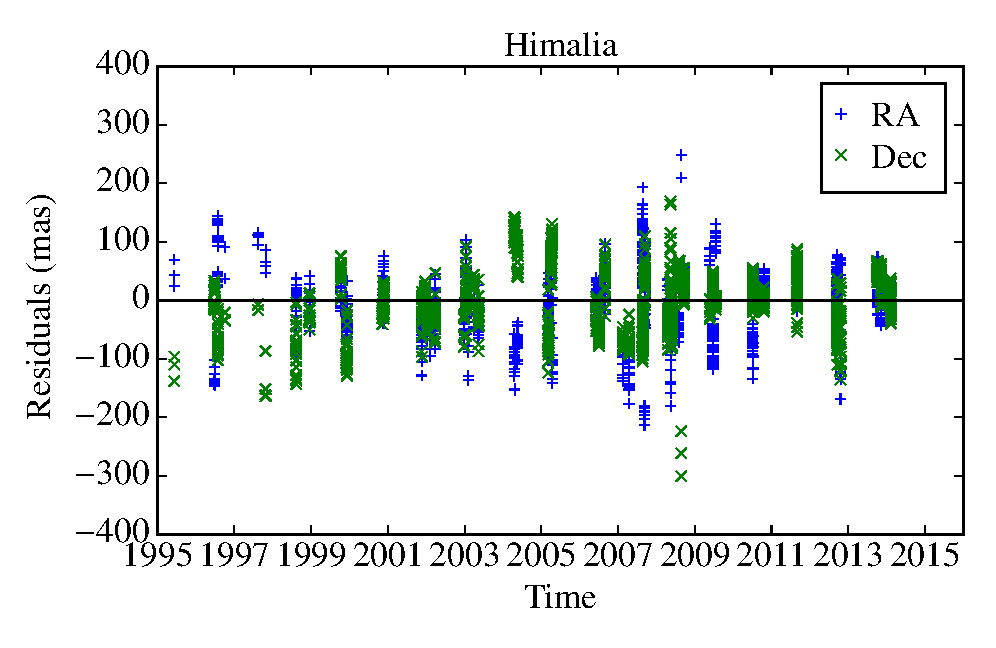
\includegraphics[width=8.8cm]{figures/Himalia_resid.eps}   \label{Fig: residuals-Himalia}}
%\subfigure{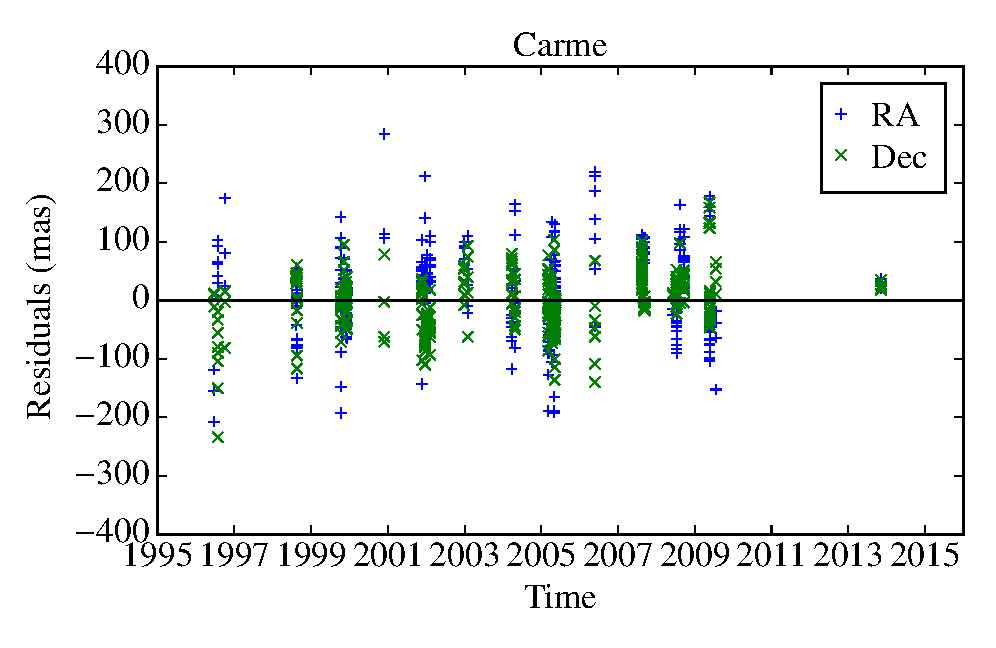
\includegraphics[width=8.8cm]{figures/Carme_resid.eps}  \label{Fig: residuals-Carme}}
%\caption{Residuals in topocentric right ascension and declination of the numerical integration for Himalia and Carme. \label{Fig: residuals}}
%\end{figure*}

%\begin{table*}
%\caption{Initial osculating elements for Jupiter irregular satellites at JD 2451545.0.% For Themisto's case, the small number of observations meant that the statistical uncertainty was even greater than the obtained elements, though the fitting proved satisfying. We decided to provide its elements with significant number comparable to the other satellite for information, but left it without uncertainty.
% }\label{Tab: sat_ell}
%\begin{center}
%\begin{tabular}{ccccccc}
%\hline\hline
%Satellite & a (km) & e & I$\degr$ & $\Omega\degr$ & $\omega\degr$ & $v\degr$ \\ 
%\hline
%Himalia &   11372100 $\pm$ 500    &    0.166 $\pm$ 0.002      &   45.14 $\pm$ 0.15      &   39.77 $\pm$ 0.19      &   351.48 $\pm$ 0.46      &   97.35 $\pm$ 0.48    \\
%Elara &   11741170 $\pm$ 690  &      0.222 $\pm$ 0.002      &   28.64 $\pm$ 0.18      &   68.42 $\pm$ 0.43      &   179.82 $\pm$ 0.56      &   339.08 $\pm$ 0.82  \\
%Lysithea &   11739900 $\pm$ 1300  &      0.136 $\pm$ 0.004      &    51.12 $\pm$ 0.27     &   5.53 $\pm$ 0.52      &   53.0 $\pm$ 1.5      &   318.9 $\pm$ 2.0   \\
%Leda &   11140300  $\pm$ 4300  &     0.173  $\pm$ 0.007     &   16.15  $\pm$ 0.75    &   272.6  $\pm$ 1.7    &   212.2  $\pm$ 3.6          &   218.8  $\pm$ 3.2  \\
%Pasiphae &  23425000  $\pm$ 5000    &     0.379  $\pm$ 0.001       &   152.44 $\pm$ 0.10      &   284.59 $\pm$ 0.21      &   135.96 $\pm$ 0.19      &   236.97 $\pm$ 0.16 \\
%Sinope &   22968800 $\pm$ 5200   &     0.316 $\pm$ 0.002      &   157.76 $\pm$ 0.12      &   256.62 $\pm$ 0.55      &   298.38 $\pm$ 0.55      &   167.57 $\pm$ 0.19    \\
%Carme &   24202924 $\pm$ 4800      &  0.242 $\pm$ 0.001      &   147.13 $\pm$ 0.10      &   154.01 $\pm$ 0.25      &   47.90 $\pm$ 0.29      &   234.41 $\pm$ 0.19  \\
%Ananke &  21683800  $\pm$ 7200  &     0.380 $\pm$ 0.002      &   172.29 $\pm$ 0.20      &   56.9 $\pm$ 1.2      &   123.3 $\pm$ 1.2      &   231.24 $\pm$ 0.21  \\
%%Themisto  & 7393800    &     0.198       &   25.77  &   220.0     &   216.3    &   262.1     \\
%\hline
%\end{tabular} 
%\end{center}
%\textbf{Notes}: a: semimajor axis; e : excentricity; I: inclination relative to the equatorial reference plane J2000; $\Omega$: longitude of the ascending node; $\omega$: argument of periapsis; $v$: true anomaly.
%\end{table*}

All the orbits determined for the satellites show satisfying residuals. %Yet, one of the satellites has a peculiar situation. Its small number of observations in our set means that its orbit is definitely loosely constrained. 
The residuals are smaller than those obtained with JPL ephemeris, which was expected because the accuracy of an ephemeris decreases when we get further from the time of observations. The main risk of divergence over time comes from the possible absence of long-term effects when fitting to a short timespan of observations. If that were the case, our ephemeris would diverge too quickly to be of any use. JPL ephemerides are fitted over all the available observations. As a result, they will diverge less quickly than our own. Though they are no longer precise enough for our use, they remain a precious reference to identify whether our own model presents a quick divergence.

We compared our ephemeris to the JPL for all the Jupiter satellites we fitted, until 2018. For instance, the divergence between 2015 and 2018 is at most 98 mas in $\Delta \alpha \cos \delta$ and 58 mas in $\Delta \delta$ for Himalia and 181 mas in $\Delta \alpha \cos \delta$ and 152 mas in $\Delta \delta$ for Carme.

Fig. \ref{Fig: JPL-STE} displays the offsets of the positions published by \cite{GomesJunior2015} for the satellite Carme in declination relative to our ephemeris, to \cite{Jacobson2012} JUP300 JPL ephemeris and \cite{Emelyanov2008} ephemeris.We see that the systematic JPL ephemeris offsets pointed out by \cite{GomesJunior2015} are reduced with our ephemeris, as expected.

\begin{figure}
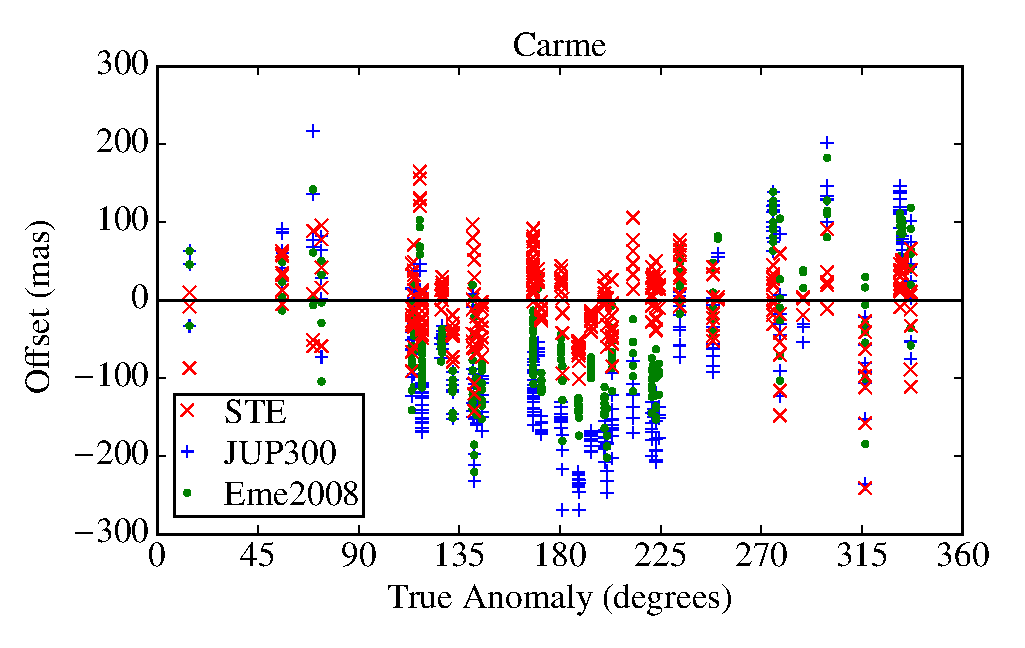
\includegraphics[width=8.8cm]{figures/Carme_ephemeris.eps} 
\caption{Offsets in declination of the positions published by \cite{GomesJunior2015} for Carme. The red "x" relative to the special-tailored ephemeris, the blue "+" relative to the JUP300 JPL ephemeris and the green dot relative to \cite{Emelyanov2008}. As expected, the ephemeris systematic errors pointed out by \cite{GomesJunior2015} are reduced with the STE ephemeris.  \label{Fig:JPL-STE}}
\end{figure}

%\begin{figure*}
%\subfigure{\includegraphics[width=8.8cm]{figures/JPL_DEC_Himalia.eps}    \label{Fig: JPL-STE-Himalia}}
%\subfigure{\includegraphics[width=8.8cm]{figures/JPL_DEC_Carme.eps}  \label{Fig: JPL-STE-Carme}}
%\caption{Geocentric right ascension and declination differences between the JUP300 JPL ephemeris and the special-tailored ephemeris for Himalia and Carme. \label{Fig: JPL-STE}}
%\end{figure*}

The obtained ephemeris is hereafter refered as STE, for special-tailored ephemeris.

\subsection{Phoebe's ephemeris}

For the specific case of Phoebe, the ninth satellite of Saturn, we have updated the ephemeris published in \cite{Desmars2013}. The new ephemeris (PH15) used the same dynamical model, including the perturbations of the Sun and the eight planets, the eight major satellites of Saturn and the $J_2$ parameter. The observations used to fit the model are identical to \cite{Desmars2013} (including 223 Cassini observations) with additional observations from \cite{GomesJunior2015}, \cite{Peng2015}, observations from Minor Planet Circulars between 2012 and 2014 (available on the Natural Satellite Data Center\footnote{\url{http://lnfm1.sai.msu.ru/neb/nss/bsapoouf.htm}}), and observations from Flagstaff \citep{NOFS} between 2012 and 2014. It represents a total number of 5886 observations from 1898 to 2014.

In Fig. \ref{Fig:eph-Phoebe} we compare our ephemeris (PH15) with the SAT375 JPL\footnote{Jacobson, R.A. 2015-Feb-27. "Satellite Ephemeris: SAT375", JPL Satellite Ephemeris File Release, \url{ftp://ssd.jpl.nasa.gov/pub/eph/satellites/nio/LINUX_PC/sat375l.txt}} and the \cite{Emelyanov2007} ephemeris. We can see that our ephemeris is closer to the SAT375 JPL ephemeris where the difference between them is smaller than 20 mas (< 10 mas in Declination). This difference is smaller than the apparent diameter of Phoebe (see Table \ref{Tab: satellite-diameter})

\begin{figure}
\begin{centering}
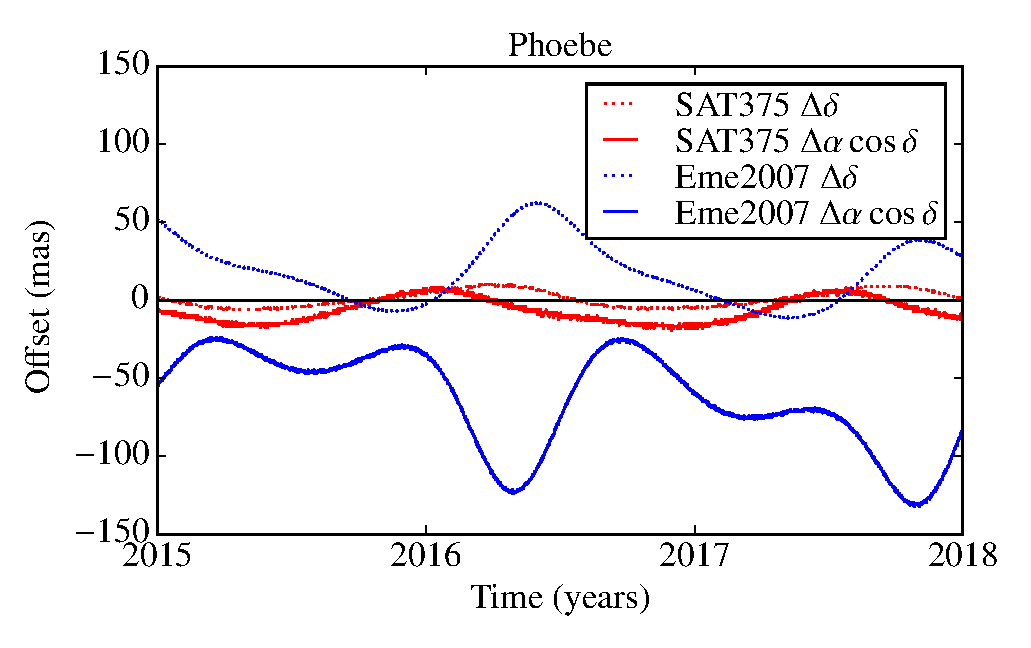
\includegraphics[width=8.8cm]{figures/Phoebe.eps} 
\caption{Comparison between the PH15, SAT375 JPL and \cite{Emelyanov2007} ephemeris for the satellite Phoebe.}
\label{Fig:eph-Phoebe}
\end{centering}
\end{figure}

\subsection{Triton's and Nereid's ephemeris}

For Triton, we used the most recent ephemeris published by \cite{Emelyanov2015}. In Fig. \ref{Fig:eph-Triton} we compare it with the ephemeris published in \cite{Zhang2014} and the NEP081 JPL ephemeris \citep{Jacobson2009}. The offsets between the three ephemeris are smaller than 15 mas for the period 2015-2018. This value is much smaller than the apparent size of Triton (124 mas, see Table \ref{Tab: satellite-diameter}), which indicates a good probability of observing an event by this object.

\begin{figure*}
\begin{centering}
\subfigure[NEP081 JPL and \cite{Emelyanov2015}]{\includegraphics[width=8.8cm]{figures/JPL-EME_Triton.eps} \label{Fig:eph-Triton-eme}}
\subfigure[\cite{Zhang2014} and \cite{Emelyanov2015}]{\includegraphics[width=8.8cm]{figures/Zhang-EME.eps} \label{Fig:eph-Triton-zhang}}
\caption{Comparison between the \cite{Emelyanov2015}, \cite{Zhang2014} and NEP081 JPL \citep{Jacobson2009} ephemeris for the satellite Triton.}
\label{Fig:eph-Triton}
\end{centering}
\end{figure*}

For Nereid, we used the ephemeris published by \cite{Emelyanov2011}, which uses more recent observations than the JPL ephemeris published by \cite{Jacobson2009}. The comparison between the two ephemeris can be seen in Fig. \ref{Fig:eph-Nereid}. The right ascension offsets between them are smaller than 60 mas and the declination ones are smaller than 15 mas. For Nereid, ephemeris errors in right ascension translate to uncertainties in the central instant of a stellar occultation, so offsets of 60 mas are not critical. The declination ephemeris offsets are of the order of the apparent diameter (15 mas, see Table \ref{Tab: satellite-diameter}), resulting in fair chances (50\%) that the shadow crosses the expected Earth latitude predicted for an occultation. % which is bigger than the satellite apparent diameter (see Table \ref{Tab: satellite-diameter}). Although this fact, the difference is bigger in Right Ascension than in Declination, which means that, in an event, the error would be smaller in the latitude where the shadow will pass on Earth than the error at the time of the occultation.

\begin{figure}
\begin{centering}
\includegraphics[width=8.8cm]{figures/JPL-EME_Nereid.eps}
\caption{Comparison between the \cite{Emelyanov2011} and NEP081 JPL \citep{Jacobson2009} ephemeris for the satellite Nereid.}
\label{Fig:eph-Nereid}
\end{centering}
\end{figure}

\cite{GomesJunior2015} published 902 new positions for Nereid from observations between 1992 and 2014. The development of a better ephemeris for Nereid using these new positions in the context discussed here of near future stellar occultations is desirable, but is out of the scope of this paper.  

%Making a new model for the orbits of these objects would demand a lot of time and delay the publication of predictions of possible events to occur in the very near future. Thus, we utilized the positions obtained by \cite{GomesJunior2015} to identify error patterns in the ephemeris. The error patterns in right ascension and in declination could be used to extrapolate the offsets to the satellite ephemeris by the time of the predicted occultation, improving it. Plots of the offsets over true anomaly (see Fig. \ref{Fig:offxanom} for declination offsets of Carme, for instance) clearly show the systematic errors in the JPL ephemeris.

%\begin{figure}
%\begin{centering}
%\includegraphics[scale=0.25]{figures/DEC.png}\label{Fig:offxtime}
%\caption{Offsets of the declination of Carme by time. \textcolor{red}{Figura só para visualização, vou colocar alguma melhor depois}}
%\end{centering}
%\end{figure}

%\begin{figure*}
%\begin{centering}
%\subfigure[Offset from the JPL ephemeris]{\includegraphics[width=8.8cm]{figures/DEC_anom.png} \label{Fig:offxtanomxjpl}}
%\subfigure[\textcolor{red}{Offset from the numerical integration}]{\includegraphics[width=8.8cm]{figures/DEC_anom.png} \label{Fig:offxtanomxni}}
%\caption{Offsets of the declination of Carme by true anomaly from the JPL ephemeris and \textcolor{red}{from the numerical integration of the positions obtained in \cite{GomesJunior2015}}.
%\label{Fig:offxanom}}
%\end{centering}
%\end{figure*}


%The two kinds of error or offset patterns adopted depending on the case are given by Eqs. \ref{eq:linear} and \ref{eq:seno}:
%
%\begin{equation}
%F(t,f) = p[0]\times t + p[1]\times \sin(f) + p[2]\times\cos(f) + p[3],
%\label{eq:linear}
%\end{equation}
%
%\begin{equation}
%\begin{split}
%%F = \{F_{x} \in  F_{c} &: (|S| > |C|) \\
%% &\quad \cap (\text{minPixels}  < |S| < \text{maxPixels}) \\
%% &\quad \cap (|S_{\text{conected}}| > |S| - \epsilon) \}
%F(t,f) = p[0]\times\sin\left(\frac{2\pi}{p[1]}\times t + p[2]\right) + p[3]\times\sin(f) + \\ +p[4]\times\cos(f) + p[5],
%\end{split}
%\label{eq:seno}
%\end{equation}
%where $F(t,f)$ is the offset obtained, $t$ is time in years counting from J2000.0 and $f$ is the true anomaly. The patterns could be applied for right ascension as well as for declination ephemeris offsets.